\documentclass[xetex,mathserif,serif]{beamer}
\usepackage{polyglossia}
\setdefaultlanguage[babelshorthands=true]{russian}
\usepackage{minted}
\usepackage{tabu}
\usepackage{pgfplots}
\usepackage{textpos}
\usepackage{subcaption}
\usepackage{graphicx}
\usepackage[normalem]{ulem}
\usepackage{algorithm2e}
\usepackage{algorithmic}
\usepackage{float}
\usepackage{amsmath}
\useoutertheme{infolines}

\usepackage{fontspec}
\setmainfont{FreeSans}
\newfontfamily{\russianfonttt}{FreeSans}

\usepackage{forest}
\usetikzlibrary{arrows}

\definecolor{links}{HTML}{2A1B81}
\hypersetup{colorlinks,linkcolor=,urlcolor=links}

\newcommand{\attribution}[1] {
	\vspace{-5mm}\begin{flushright}\begin{scriptsize}\textcolor{gray}{\textcopyright\, #1}\end{scriptsize}\end{flushright}
}

\tabulinesep=0.7mm

\title{Автоматы и лексический анализ}
\author[Юрий Литвинов]{Юрий Литвинов \newline \textcolor{gray}{\small\texttt{yurii.litvinov@gmail.com}}}

\date{10.12.2019}

\begin{document}
	
	\frame{\titlepage}

	\section{Работа компилятора}

	\begin{frame}
		\frametitle{Напоминание о процессе компиляции C++-кода}
		\begin{center}
			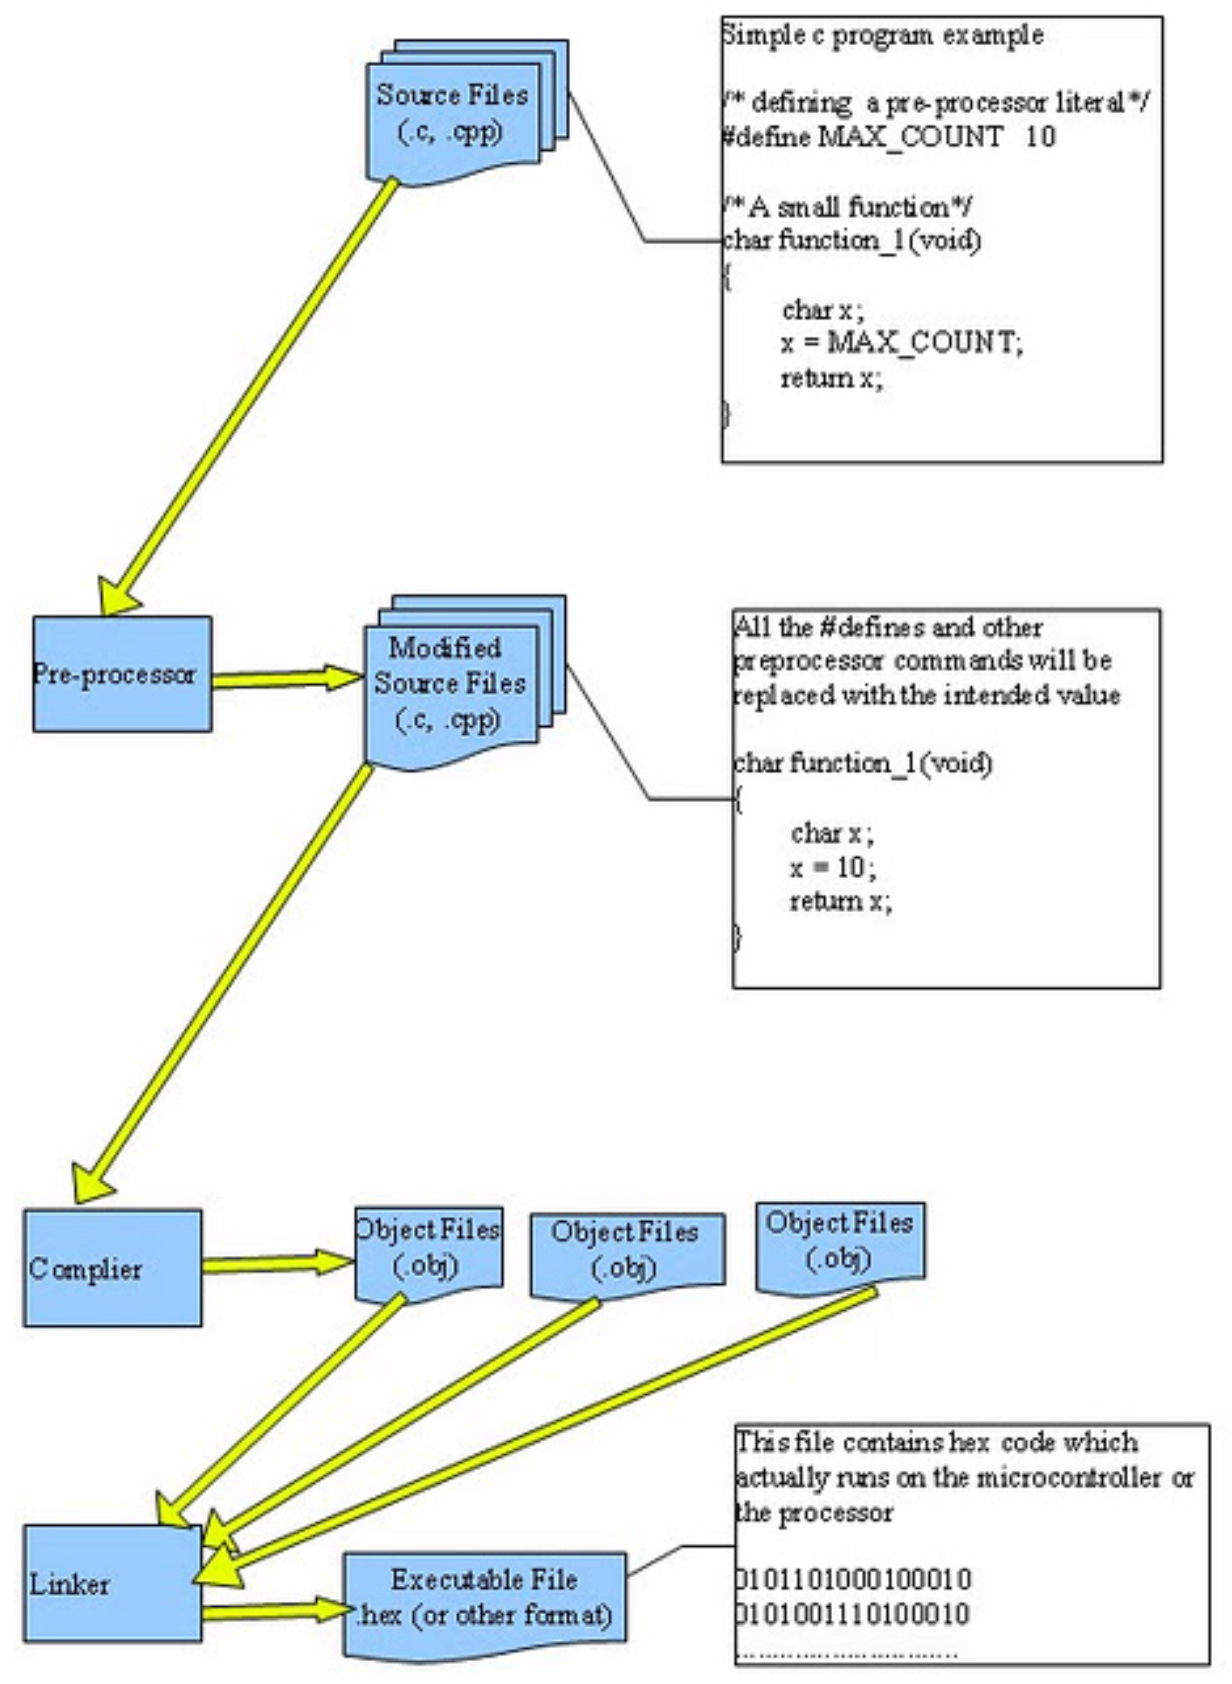
\includegraphics[height=0.8\textheight]{cppCompilation.png}
		\end{center}
	\end{frame}

	\begin{frame}
		\frametitle{Фазы компилятора}
		\begin{center}
			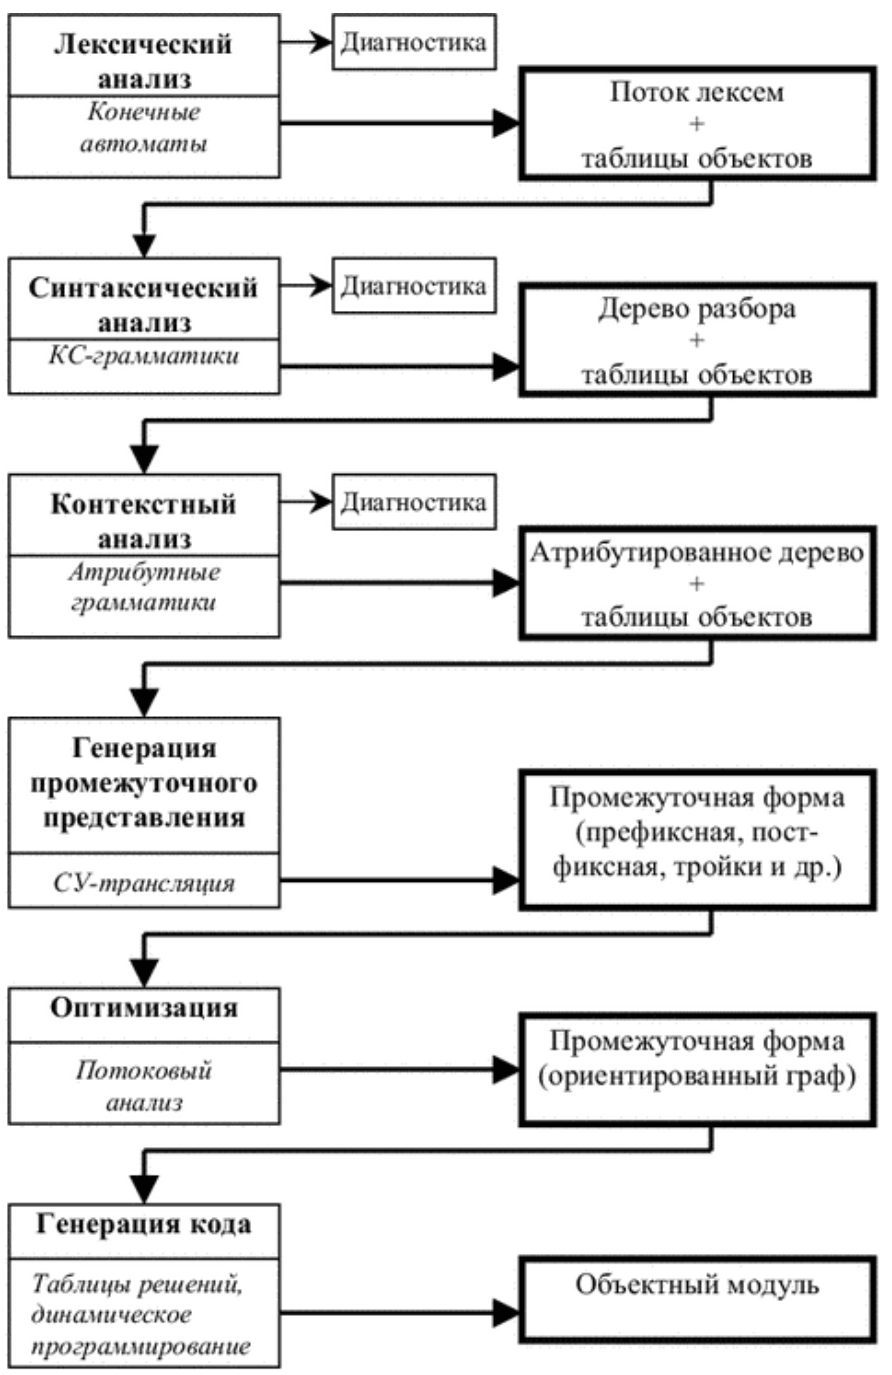
\includegraphics[height=0.8\textheight]{compilerPhases.png}
		\end{center}
	\end{frame}

	\begin{frame}
		\frametitle{Лексический анализ}
		\begin{itemize}
			\item Преобразование потока символов в поток токенов
			\item Например, \mintinline{text}|position := initial + rate * 60|
			\begin{itemize}
				\item Идентификатор position
				\item Символ присвоения
				\item Идентификатор initial
				\item Знак сложения
				\item Идентификатор rate
				\item Знак умножения
				\item Число 60
			\end{itemize}
			\item Токен представляется в виде структуры из типа токена и его значения
		\end{itemize}
	\end{frame}

	\section{Формальные языки}

	\begin{frame}
		\frametitle{Формальные языки, определения}
		\begin{itemize}
			\item Алфавит --- произвольное множество. Элементы множества называются \textit{символами} алфавита.
			\item Строка (она же \textit{цепочка}) --- конечная последовательность символов из алфавита.
			\item Длина строки $s$ (обозначается как $\lvert{s}\rvert$) --- количество символов в строке.
			\item Пустая строка ($\epsilon$) --- строка, которая не содержит символов.
			\item Конкатенация строк --- две строки, записанные друг за другом.
			\item Язык --- множество строк. Например, пустой язык (обозначается $\{\}$), множество всех корректных 
				программ на С++, множество всех грамматически корректных предложений русского языка.
		\end{itemize}
	\end{frame}

	\begin{frame}
		\frametitle{Операции над языками}
		\framesubtitle{Позволяют собрать из простых более сложные}
		\begin{itemize}
			\item Объединение $L$ и $M$ ($L \cup M$) --- $L \cup M = \{s \mid s \in L \vee s \in M\}$
			\item Конкатенация $L$ и $M$ ($LM$) --- $LM = \{st \mid s \in L \wedge t \in M\}$
			\item Замыкание Клини или \textit{итерация} (она же \textit{звёздочка Клини}) ($L^*$) --- 
				$L^* = \bigcup\limits_{i=0}^{\infty}L^i$, где $L^i$ --- это $LL \ldots L$ $i$ раз
			\begin{itemize}
				\item В том числе, $i = 0$, то есть $\epsilon$ всегда принадлежит $L^*$
				\begin{itemize}
					\item То есть, пустая строка всегда часть замыкания
				\end{itemize}
			\end{itemize}
			\item Позитивное замыкание $L$ ($L^+$) --- $LL^*$
			\begin{itemize}
				\item Или $L^* = \bigcup\limits_{i=1}^{\infty}L^i$, то есть замыкание без пустой строки
			\end{itemize}
		\end{itemize}
	\end{frame}

	\begin{frame}
		\frametitle{Регулярные выражения}
		\framesubtitle{Формальный язык для записи языков}
		\begin{itemize}
			\item Регулярное выражение $\epsilon$ задаёт язык $\{\epsilon\}$
			\item Регулярное выражение $a$ задаёт язык $\{a\}$ (язык из одного символа)
			\item Пусть $r$ и $s$ --- регулярные выражения, задающие языки $L(r)$ и $L(s)$. Тогда
			\begin{itemize}
				\item Регулярное выражение $(r) \mid (s)$ задаёт объедиение, $L(r) \cup L(s)$
				\item Регулярное выражение $(r)(s)$ задаёт конкатенацию, $L(r)L(s)$
			\end{itemize}
			\item Регулярное выражение $(r)^*$ задаёт замыкание Клини, $(L(r))^*$
			\item Регулярное выражение $(r)$ задаёт $L(r)$ (то есть можно ставить скобки)
			\item Регулярное выражение $r?$ задаёт $L(r) \cup \epsilon$
			\item Регулярное выражение $r+$ задаёт $L(r)^+$
			\item Регулярное выражение $[a..z]$ задаёт $L(a) \cup L(b) \cup \ldots \cup L(z)$
		\end{itemize}
	\end{frame}

	\begin{frame}
		\frametitle{Регулярные определения}
		\framesubtitle{Именуем регулярные выражения для удобства записи}
		\begin{itemize}
			\item $letter \rightarrow A | B | ... | Z | a | b | ... | z$
			\item $digit \rightarrow 0 | 1 | ... | 9$
			\item $id \rightarrow letter (letter | digit)*$
			\item $num \rightarrow digit+ (. digit+)? (E(+ | -)? digit+)?$
			\item $relop \rightarrow < | <= | = | <> | > | >=$
		\end{itemize}
	\end{frame}

	\begin{frame}
		\frametitle{Диаграммы переходов}
		$relop \rightarrow < | <= | = | <> | > | >=$
		\begin{center}
			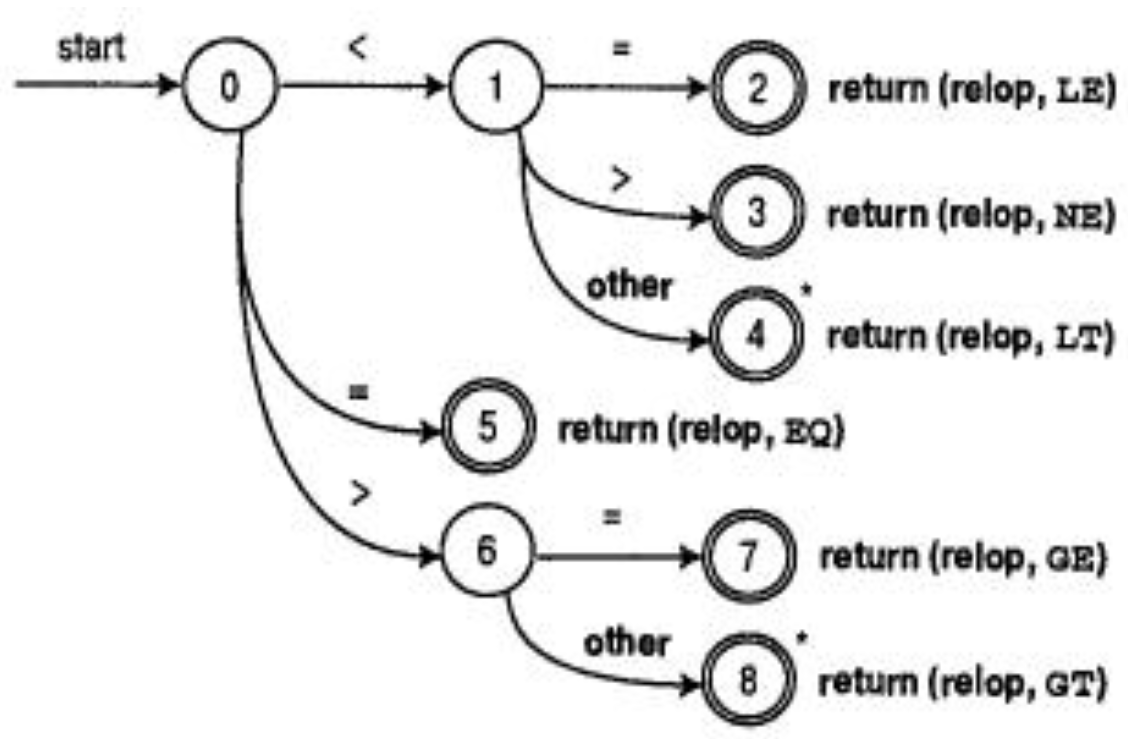
\includegraphics[height=0.5\textheight]{transitionDiagram.png}
		\end{center}
		\begin{itemize}
			\item Двойной кружок --- \textit{принимающее состояние}
			\item Звёздочка --- вернуть последний символ во входной поток
		\end{itemize}
	\end{frame}

	\begin{frame}
		\frametitle{Как это закодить}
		$relop \rightarrow < | <= | = | <> | > | >=$
		\begin{columns}
			\begin{column}{0.5\textwidth}
				\begin{center}
					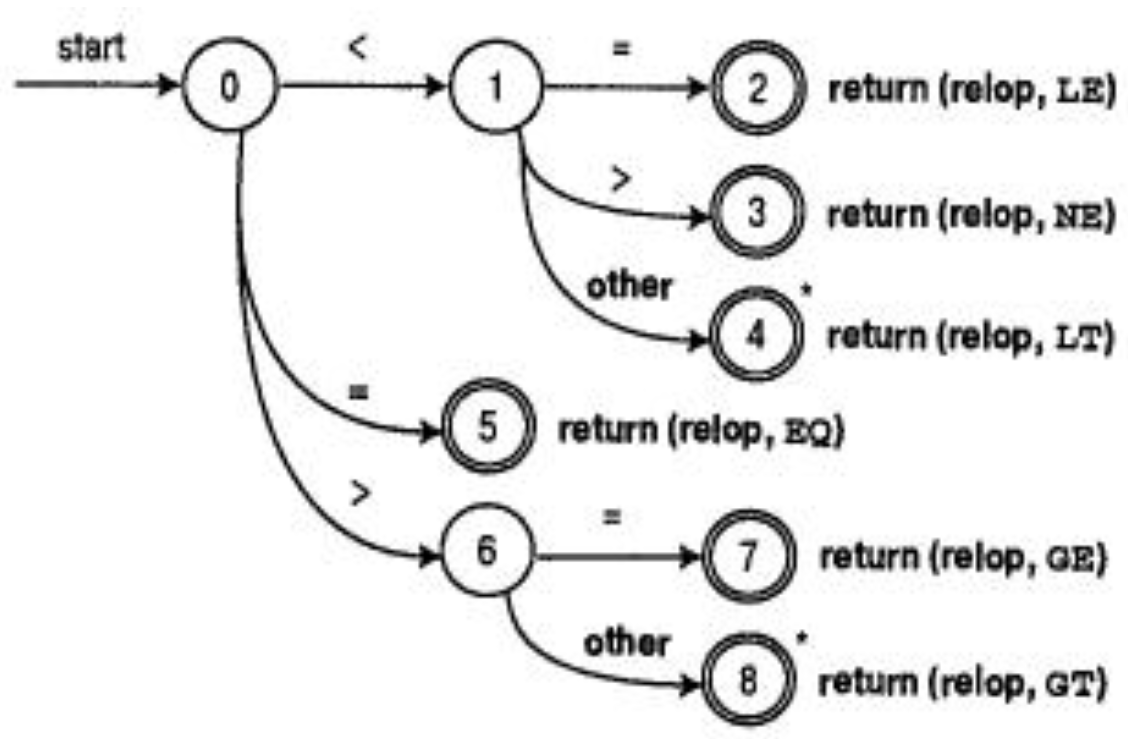
\includegraphics[width=0.9\textwidth]{transitionDiagram.png}
				\end{center}
			\end{column}
			\begin{column}{0.5\textwidth}
				\begin{center}
					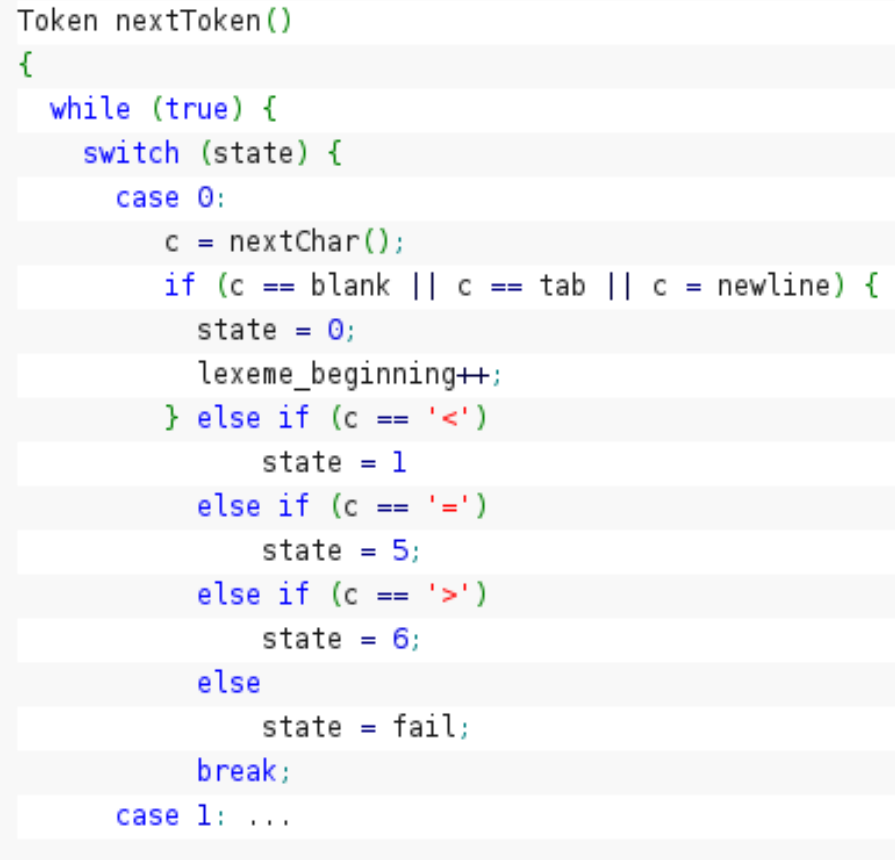
\includegraphics[width=0.9\textwidth]{lexerCode.png}
				\end{center}
			\end{column}
		\end{columns}
	\end{frame}

	\section{Автоматы}

	\begin{frame}
		\frametitle{Конечные автоматы}
		\begin{itemize}
			\item Конечный автомат --- $(S, \Sigma, move, s_0, F)$
			\begin{itemize}
				\item $S$ --- множество состояний
				\item $\Sigma$ --- входной алфавит
				\item move --- функция переходов
				\item $s_0$ --- начальное состояние
				\item $F$ --- множество допускающих состояний
			\end{itemize}
			\item Неформально автомат имеет состояние, в зависимости от которого может по-разному реагировать на входные символы (или события)
			\item Применяются не только в лексическом анализе, но и в сетевых протоколах, пользовательских интерфейсах и т.д. и т.п.
			\item Автомат принимает язык, если для любой строки языка после выполнения всех переходов он оказывается в допускающем состоянии
		\end{itemize}
	\end{frame}

	\begin{frame}
		\frametitle{ДКА и НКА}
		\begin{itemize}
			\item Детерминированный конечный автомат (ДКА) --- $move: S \times \Sigma \rightarrow S$
			\item Недетерминированный конечный автомат (НКА) --- $move: 2^S \times \Sigma \cup \epsilon \rightarrow 2^S$
			\begin{itemize}
				\item НКА может находиться в нескольких состояниях одновременно и делать переход одновременно в несколько разных состояний
				\item Или, другая точка зрения --- он не знает, в каком именно состоянии сейчас находится
				\item И есть эпсилон-переходы --- спонтанные переходы, без входного символа
			\end{itemize}
		\end{itemize}
	\end{frame}

	\begin{frame}
		\frametitle{Пример НКА}
		Пусть есть язык, задаваемый регулярным выражением $a a^* \mid b b^*$. Тогда его принимает НКА:
		\begin{center}
			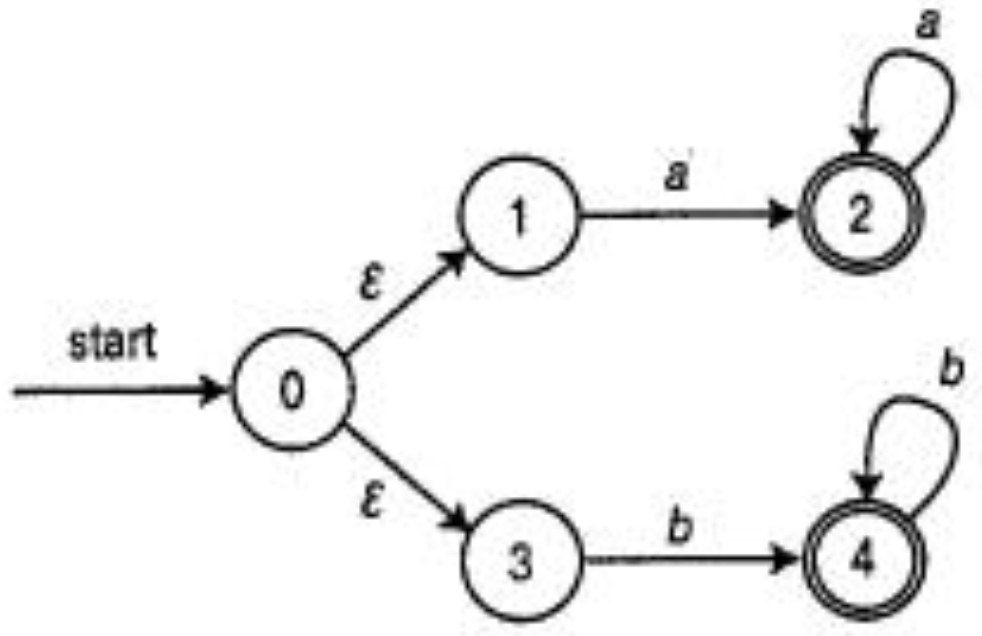
\includegraphics[height=0.6\textheight]{nfa.png}
		\end{center}
	\end{frame}

	\begin{frame}
		\frametitle{Построение НКА по регулярному выражению}
		Теорема: по любому РВ можно построить НКА, принимающий язык РВ. Доказательство:
		\begin{center}
			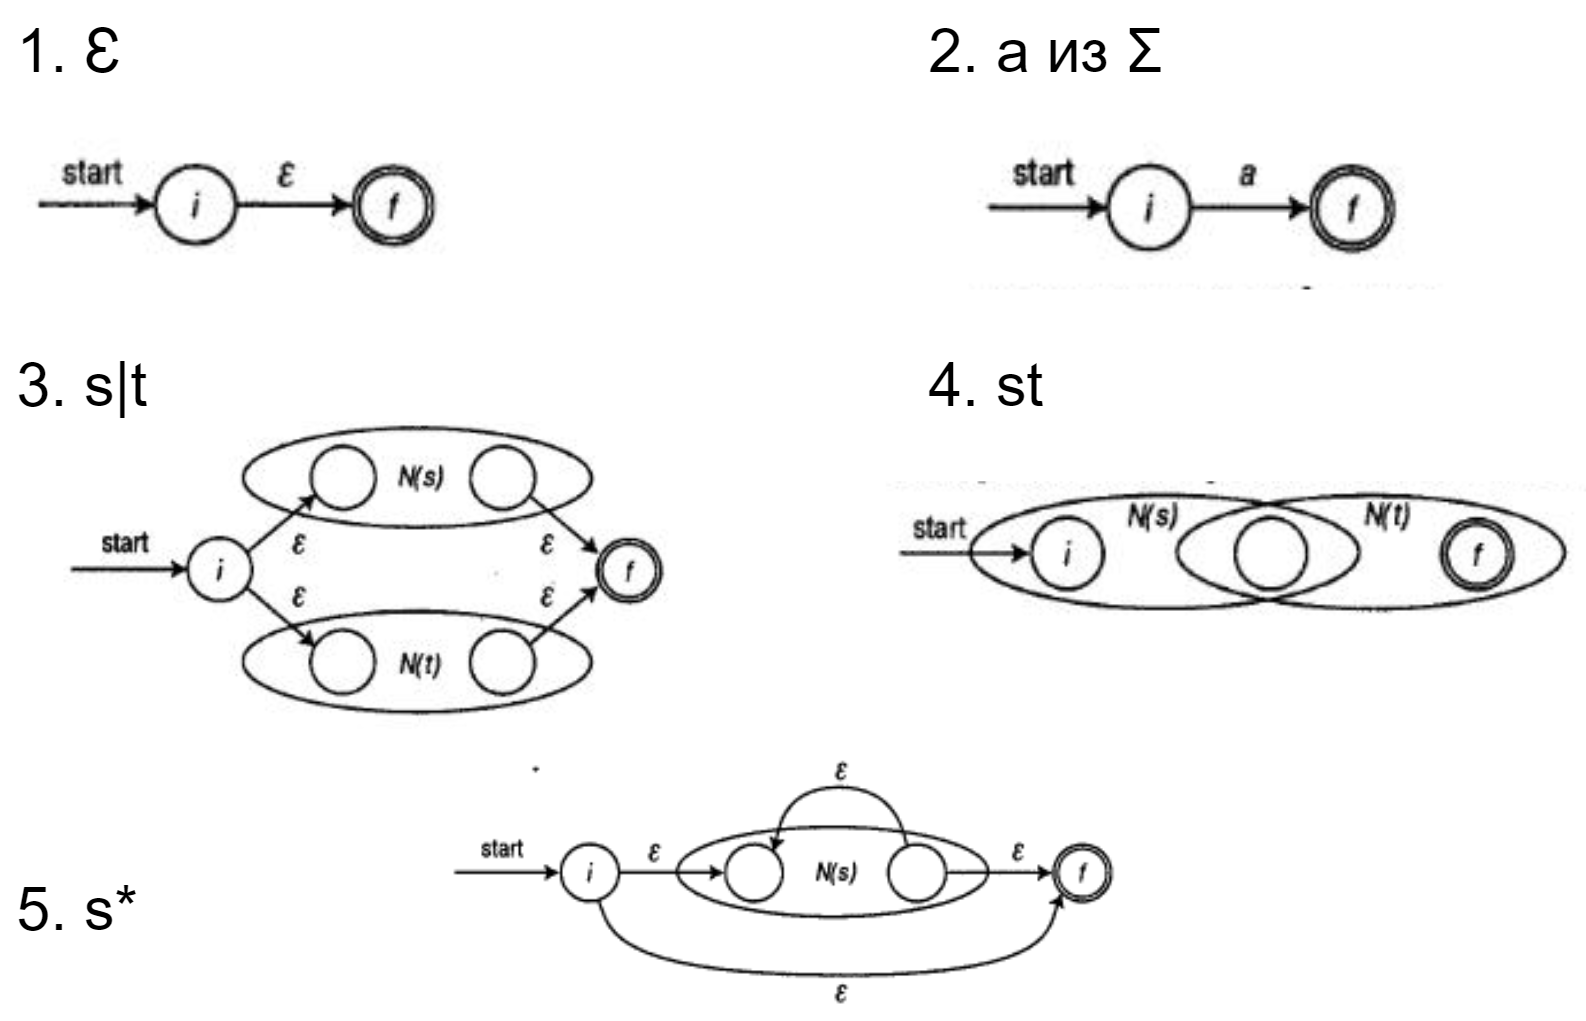
\includegraphics[height=0.6\textheight]{nfaByRegexp.png}
		\end{center}
	\end{frame}

	\begin{frame}
		\frametitle{Моделирование НКА, таблица переходов}
		\begin{center}
			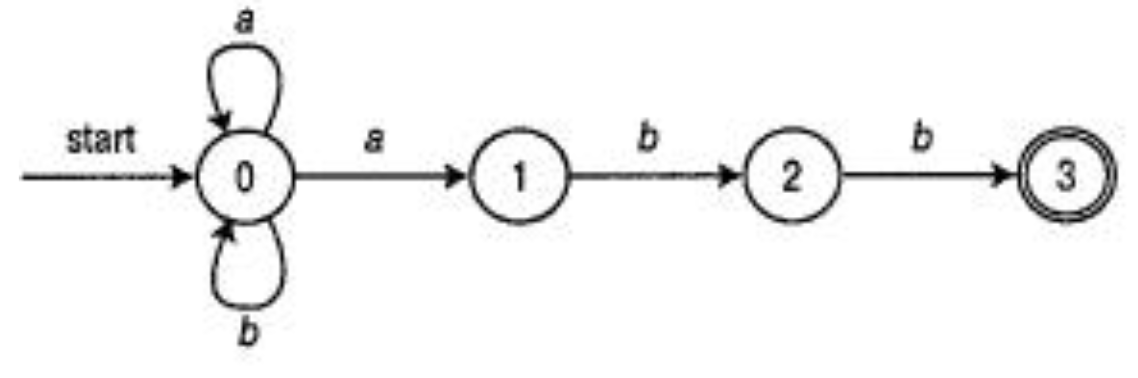
\includegraphics[width=0.8\textwidth]{abbNfa.png}
		\end{center}
		\begin{center}
			\begin{tabu} {| X[0.9 l p] | X[1 l p] | X[1 l p] |}
				\tabucline-
				Состояние              & a           & b        \\
				\tabucline-
				\everyrow{\tabucline-}
				0                      & $\{0, 1\}$  & $\{0\}$  \\
				1                      & ---         & $\{2\}$  \\
				2                      & ---         & $\{3\}$  \\
			\end{tabu}
		\end{center}
	\end{frame}

	\begin{frame}
		\frametitle{Построение ДКА по НКА}
		Теорема: по любому НКА можно построить ДКА, принимающий в точности тот же язык (то есть НКА и ДКА эквивалентны друг другу в плане выразительности).

		Без доказательства.
	\end{frame}

	\begin{frame}
		\frametitle{Пример}
		\begin{center}
			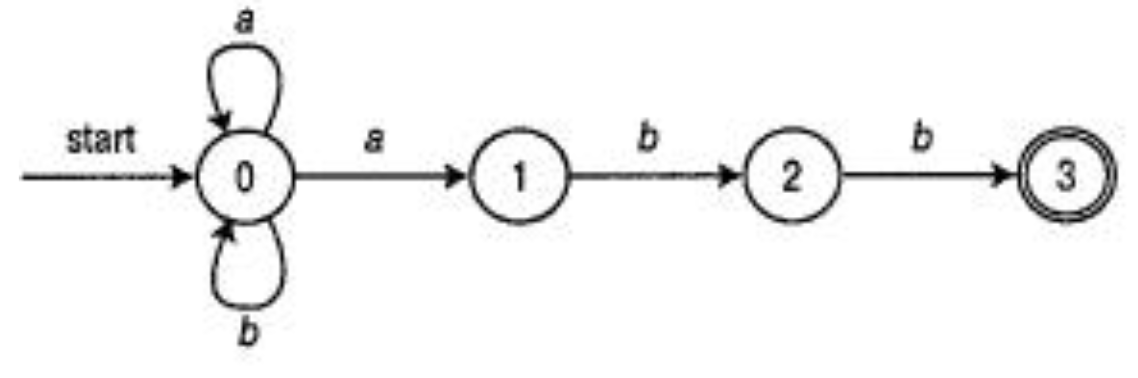
\includegraphics[width=0.7\textwidth]{abbNfa.png}
		\end{center}
		\begin{center}
			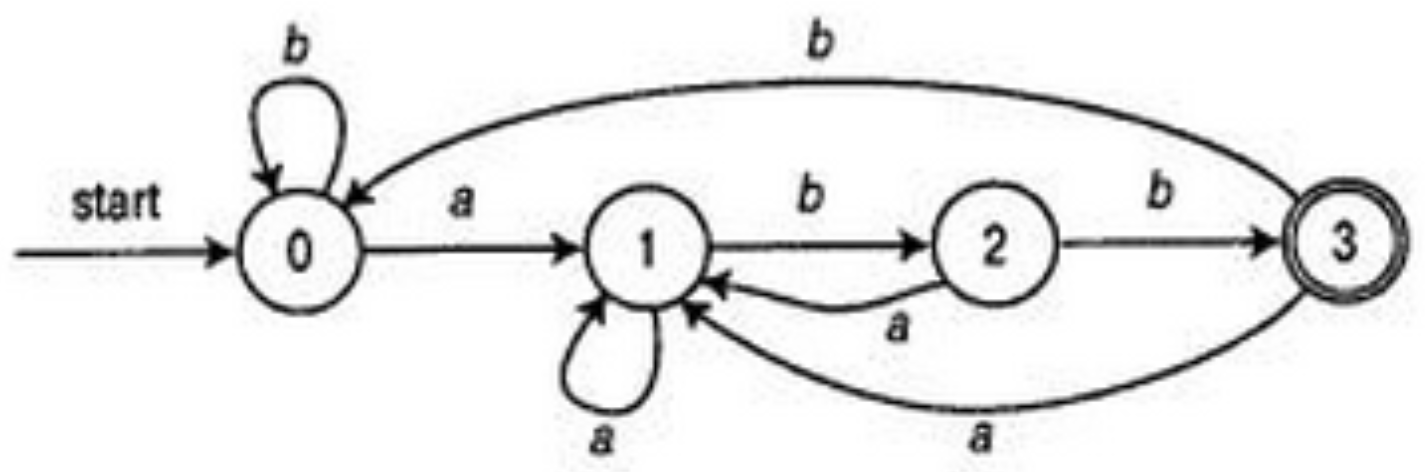
\includegraphics[width=0.7\textwidth]{abbDfa.png}
		\end{center}
	\end{frame}

	\begin{frame}
		\frametitle{Моделирование ДКА}
		\begin{center}
			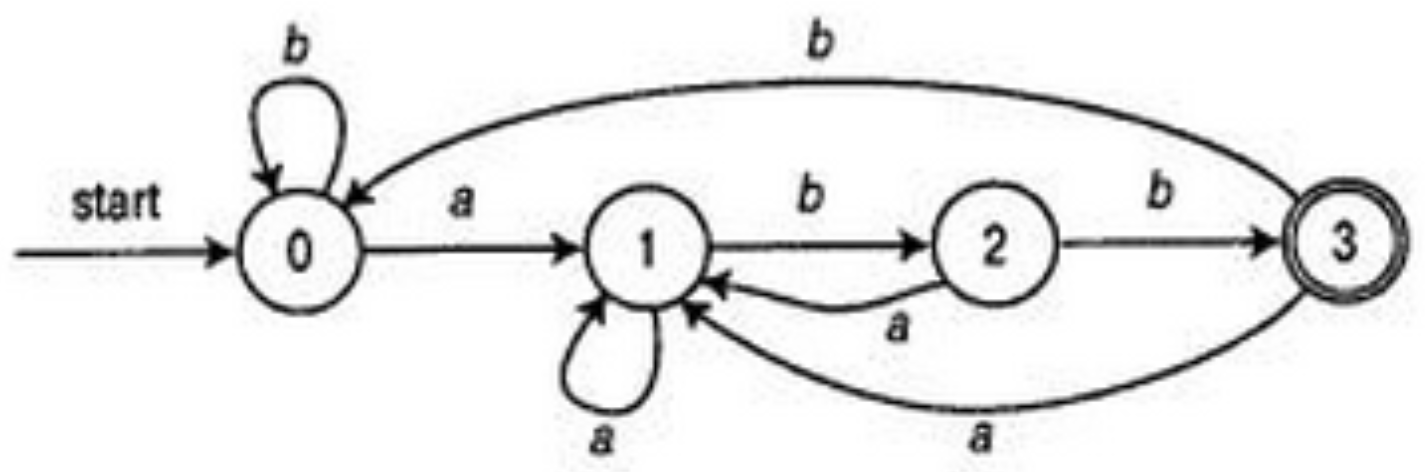
\includegraphics[width=0.7\textwidth]{abbDfa.png}
		\end{center}
		\begin{center}
			\begin{tabu} {| X[0.9 l p] | X[1 l p] | X[1 l p] |}
				\tabucline-
				Состояние              & a         & b  \\
				\tabucline-
				\everyrow{\tabucline-}
				0                      & 1         & 0  \\
				1                      & 1         & 2  \\
				2                      & 1         & 3  \\
				3                      & 1         & 0  \\
			\end{tabu}
		\end{center}
	\end{frame}

	\begin{frame}[fragile]
		\frametitle{Как это выглядит в коде}
		\begin{itemize}
			\item switch-case вполне вариант
			\item Интерпретировать таблицу состояний
			\begin{itemize}
				\item Лучше, меньше кода и гибче
			\end{itemize}
		\end{itemize}
		\begin{minted}{pascal}
while c <> eof do begin
    s := move(s, c);
    c := nextchar();
end;
if s in F then
    return true
else
    return false
		\end{minted}
	\end{frame}

	\begin{frame}
		\frametitle{Книжка}
		А. Ахо, Р. Сети, Дж. Ульман, М. Лам. Компиляторы. Принципы, технологии, инструменты.
		\begin{center}
			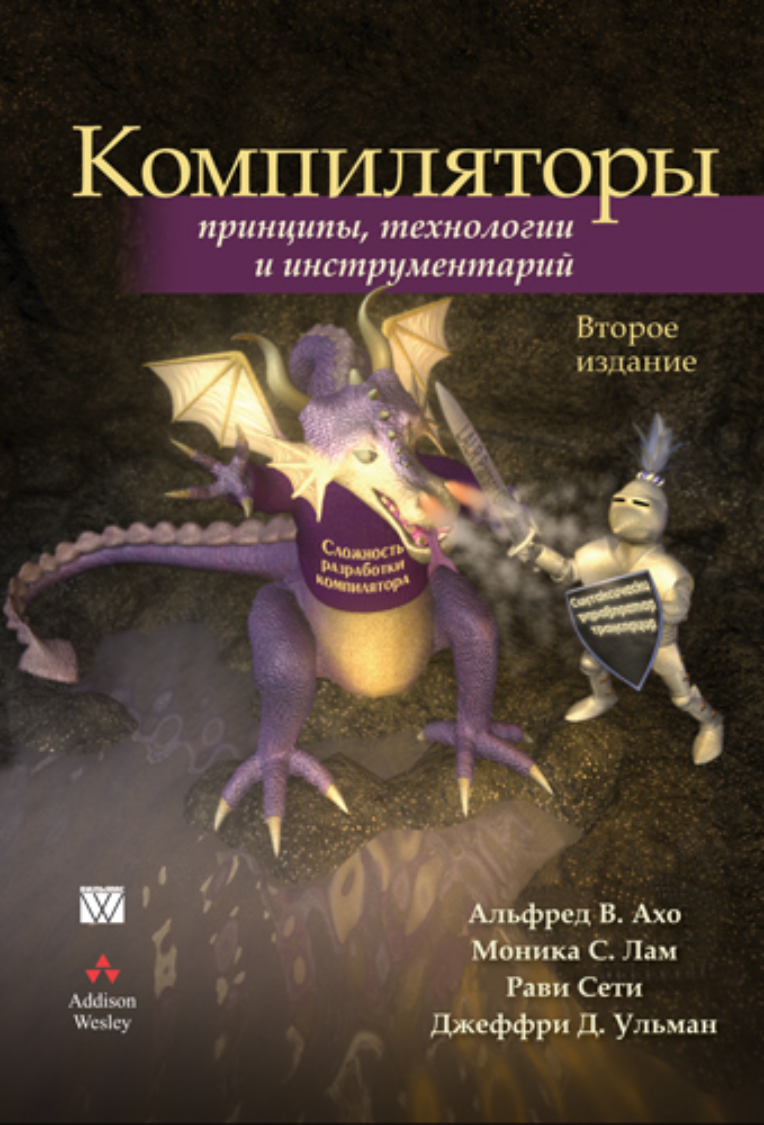
\includegraphics[width=0.25\textwidth]{compilersCover.png}
		\end{center}
	\end{frame}


\end{document}